\documentclass[aps,prl,reprint,amsfonts,amsmath,amssymb,showpacs,groupedaddress,superscriptaddress]{revtex4-1}
\usepackage{bm}
\usepackage{color}
\usepackage{graphicx}
\usepackage[colorlinks,urlcolor=blue,linkcolor=blue,anchorcolor=blue,citecolor=blue,bookmarks]{hyperref}

\begin{document}

\title{Artificial two-dimensional Mott insulating superstructures with a large Mott gap: Theoretical Formalism}

\date{\today}

\maketitle

To have a better understading of the experimental observations, we construct single-band Hubbard model with renormalized hopping coefficients to describe these systems and calculate the local density of states by using cluster perturbation theory (CPT)~\cite{PhysRevB.48.418,PhysRevLett.84.522}.

For the $(3\sqrt{7} \times 3\sqrt{7})R19.1^\circ$ surface (referred to as Phase 1 in the followings), the corresponding proposed atomic structural is shown in Fig.~\ref{fig:STMTopographicImage}(g). The unit cell contains twenty-three sites while three of them are somewhat isolated, see the three blue circles in Fig.~\ref{fig:STMTopographicImage}(d). Considering that the hopping amplitude is inversely proportional to the square of the distance, it is reasonable to neglect the three isolated sites in a simplified model. We only include these hopping terms shown in Fig.~\ref{fig:ModelForPhase1} and the resulting Hamiltonian takes the following form:
\begin{equation}
    H = \sum_{<i,j>\sigma} t_{ij}(c_{i\sigma}^{\dagger}c_{j\sigma} + \text{H.c.}) + U \sum_{i} n_{i\uparrow} n_{i\downarrow}
    \label{eq:ModelHamiltonian}
\end{equation}
where $t_{ij}$ is the effective hopping amplitude and $U$ the effective on-site Coulomb repulsion. Here, we take $t_{ij} = -1/r_{ij}^{2}$, where $r_{ij}$ is the distance between $i$-th site and $j$-site.
\textcolor{red}{See appendix for the coordinates of these sites shown in Fig.~\ref{fig:ModelForPhase1}.}

For this model Hamiltonian, we first consider the non-interacting case (\textit{i.e.,} $U = 0$). The corresponding energy band and local density of states are shown in Fig.

\begin{figure}[p]
    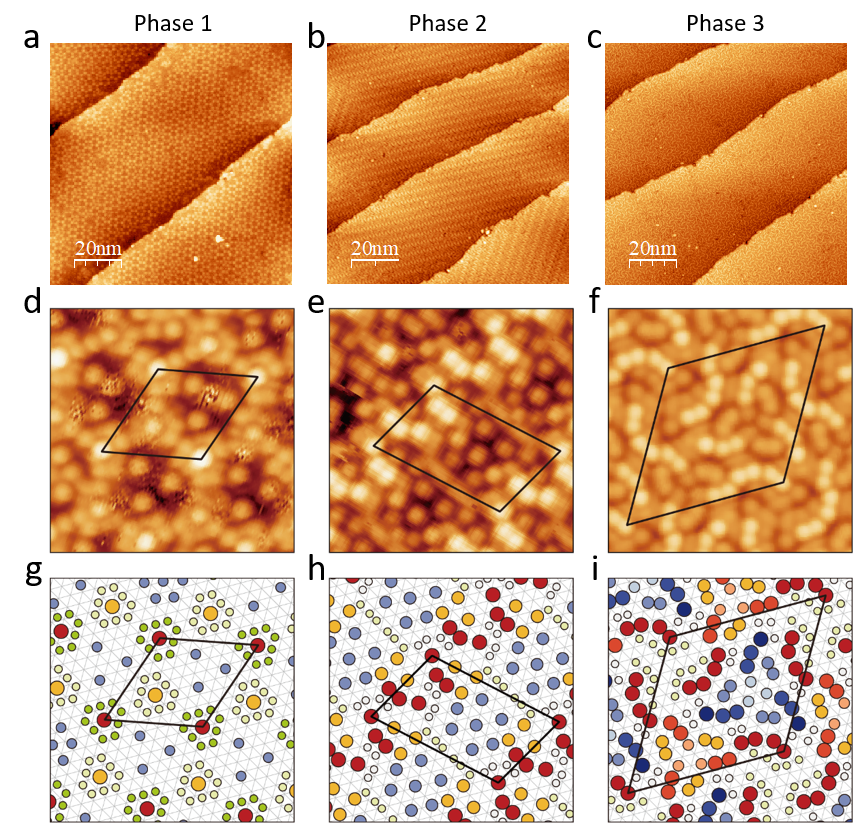
\includegraphics[width=\columnwidth]{STMTopographicImage.png}
    \caption{\label{fig:STMTopographicImage}(Color online) STM characterization of three new superstructures of Sn sub-monolayers on Si(111). (a)-(c) Large-scale STM image (size: 100 $\times$ 100 nm$^2$) taken on $(3\sqrt{7} \times 3\sqrt{7})R19.1^\circ$, $(\sqrt{133} \times 4\sqrt{3})$ and $(13 \times 13)$ surfaces. They are taken at $U = +3.5V$, $U = -2V$ and $U = -2V$ ($I_{t} = 100pA$) respectively. (d)-(f) The atomically resolved STM images of them taken at $U = -2V, I_{t} = 200pA$. The surface unit cells of them are marked in black. (g)-(i) The corresponding proposed atomic structural models. The marked surface unit cells in (g)-(i) are the same as these in (d)-(f).}
\end{figure}

\begin{figure}[p]
    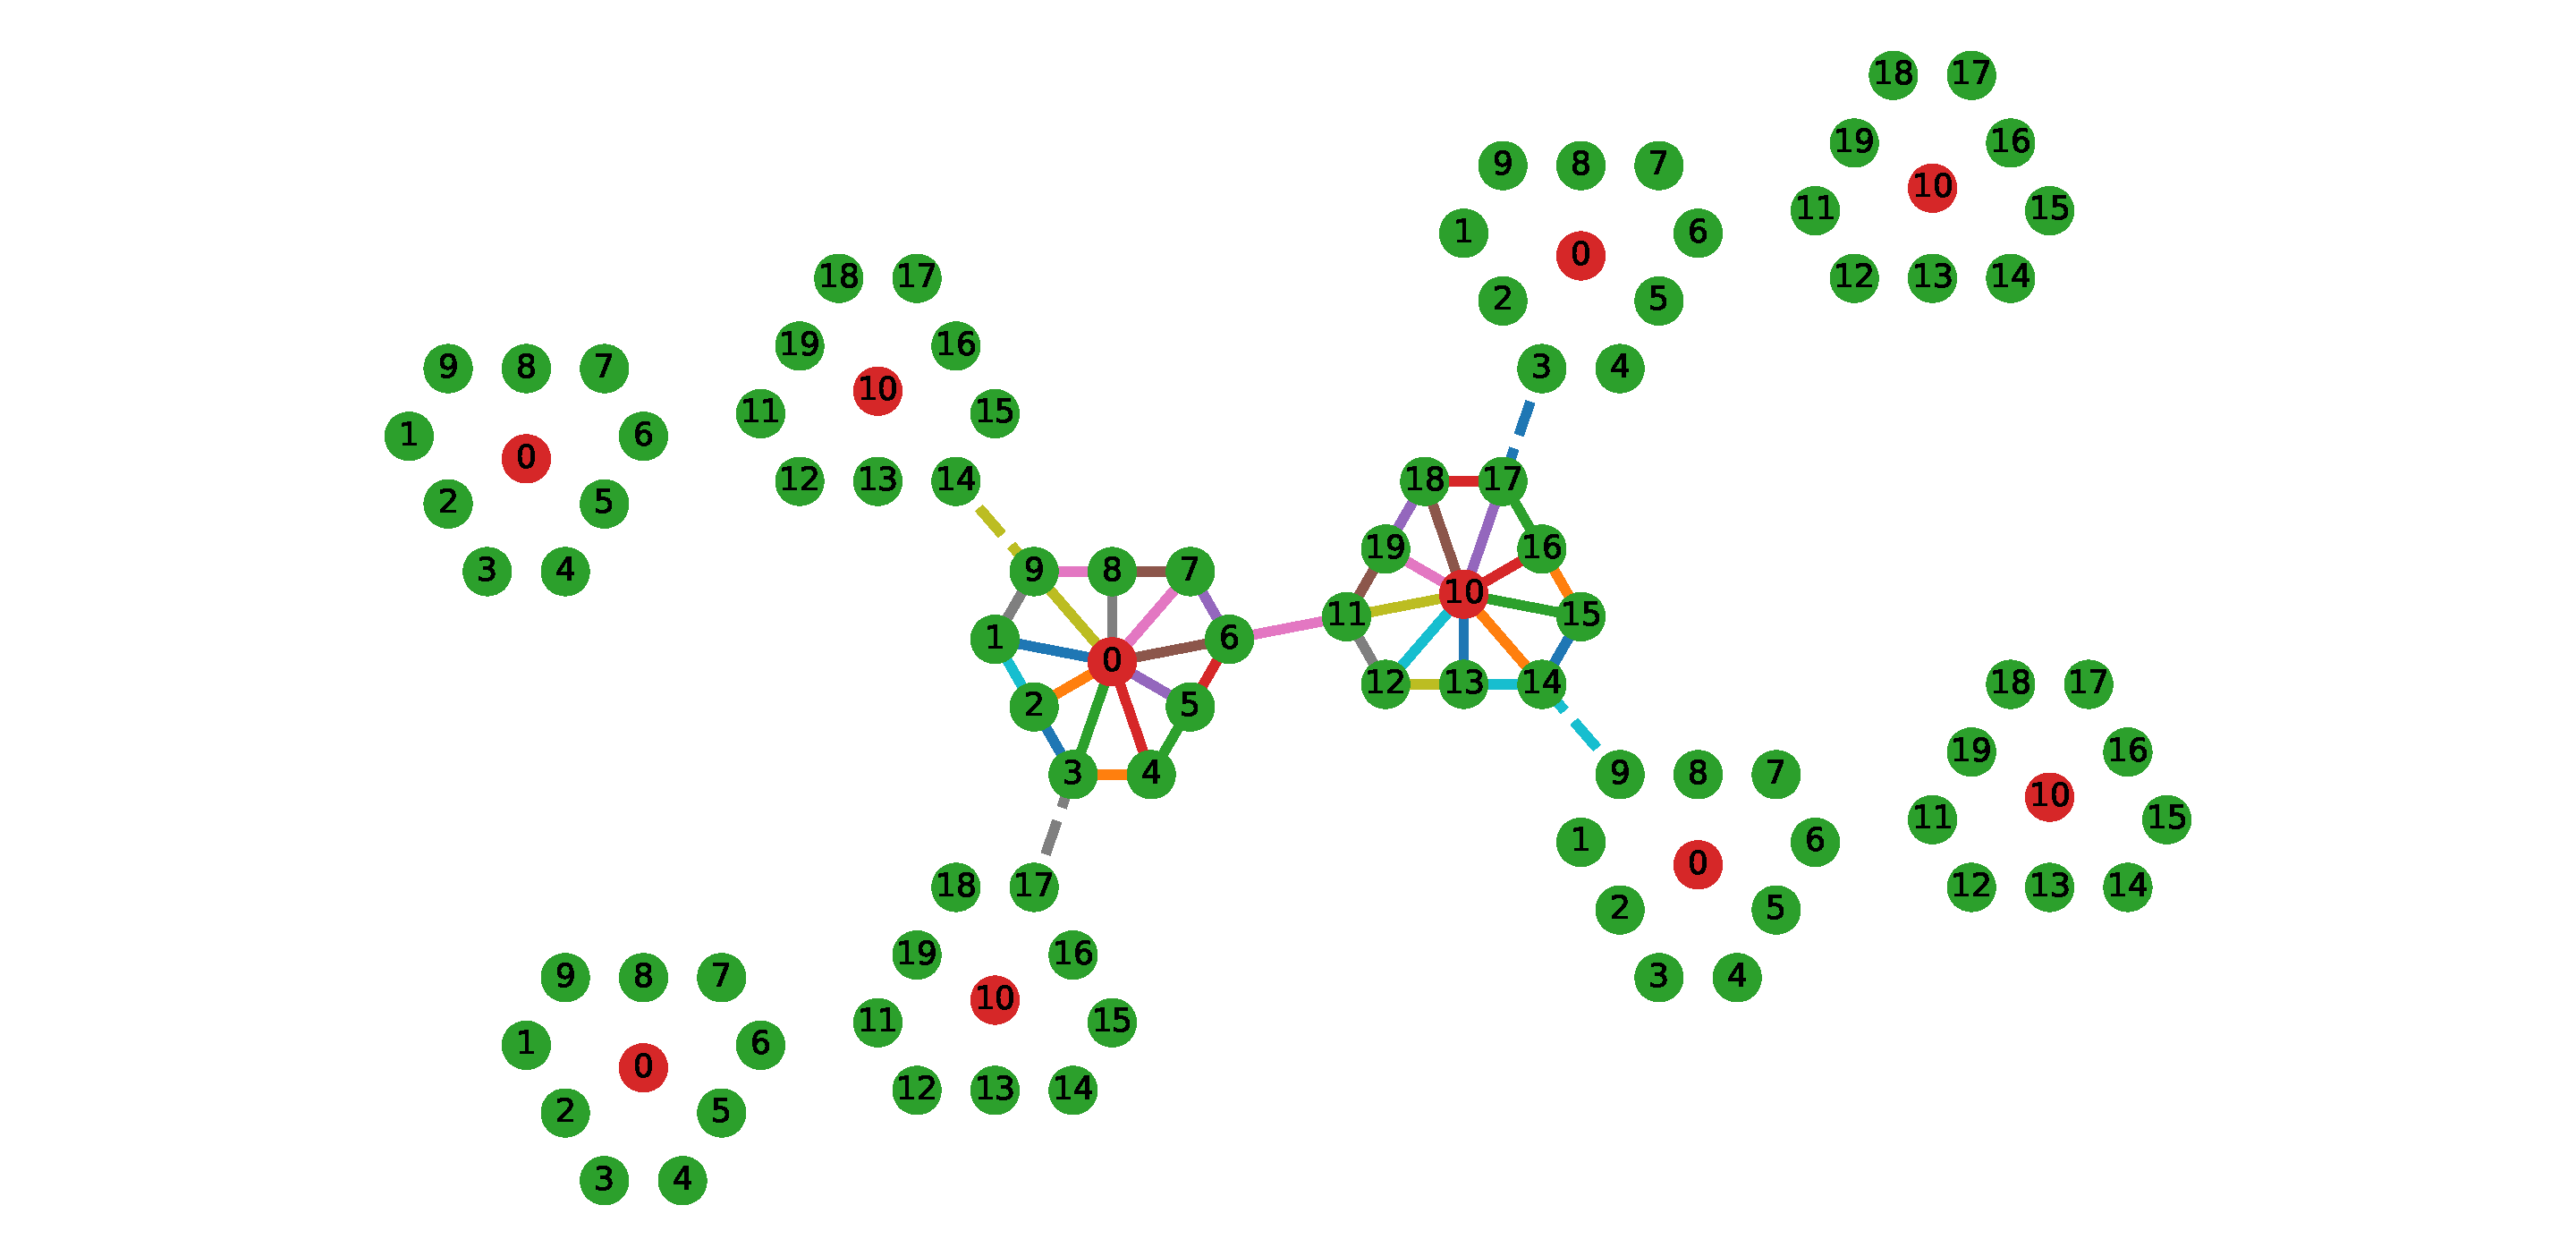
\includegraphics[width=\columnwidth]{ModelForPhase1.pdf}
    \caption{\label{fig:ModelForPhase1} (Color online) Demonstration of the hopping terms for Phase 1. The unit cell has twenty sites labeled from 0 to 19. The soild and dashed lines correspond to the hopping terms $t_{ij} (c_{i\sigma}^{\dagger} c_{j\sigma} + \text{H.c.})$, where $t_{ij} = -1/r_{ij}^{2}$ and $r_{ij}$ is the distance from $i$-th to $j$-th site.}
\end{figure}

\bibliography{TheoreticalFormalism}

\end{document}
